\documentclass[11pt,letterpaper]{article}
\usepackage[T1]{fontenc}
\usepackage[utf8]{inputenc}
\usepackage{lmodern,amsmath,amssymb,mathtools,booktabs,array,graphicx,xcolor,microtype}
\usepackage[margin=.87in,top=.82in,bottom=.83in,headheight=14pt]{geometry}
\usepackage{fancyhdr,enumitem}
\usepackage[colorlinks=true,urlcolor=teal!65!black,linkcolor=teal!65!black,citecolor=teal!65!black]{hyperref}
\definecolor{ink}{HTML}{173A44}\definecolor{sea}{HTML}{21675E}
\pagestyle{fancy}\fancyhf{}\fancyhead[L]{\small\color{ink}The solid oloid in iPRA}
\fancyhead[R]{\small\color{ink}Constructive geometry}\fancyfoot[C]{\small\thepage}
\renewcommand{\headrulewidth}{.3pt}
\newcommand{\sect}[1]{\section[#1]{\color{ink}#1}}
\newcommand{\subt}[1]{\par\medskip\noindent{\color{sea}\bfseries #1}\enspace}
\newcommand{\dd}{\mathop{}\!d}
\newcommand{\Q}{\mathbb Q}\newcommand{\N}{\mathbb N}
\newcommand{\ax}{\parallel}\newcommand{\tr}{\perp}
\newcommand{\Dth}{D_{\theta}}
\setlength{\parindent}{1.18em}\setlength{\parskip}{2pt}
\setlist{nosep,leftmargin=*}\allowdisplaybreaks
\hypersetup{pdftitle={The solid oloid in intuitionistic primitive recursive arithmetic},pdfauthor={OpenAI}}
\begin{document}
\thispagestyle{plain}
{\color{sea}\small\bfseries CONSTRUCTIVE GEOMETRY}\par\vspace{7pt}
{\color{ink}\fontsize{27}{30}\selectfont\bfseries The solid oloid in intuitionistic\\primitive recursive arithmetic}\par
\vspace{7pt}
{\large Surface area, volume, and centroidal moments of inertia}\par
\vspace{12pt}
\noindent Let two circles of radius \(r>0\) lie in perpendicular planes, with the center of each on the other. Fill their convex hull uniformly with mass density \(\rho>0\). Put the origin halfway between the centers and take their joining line as the \(x\)-axis. Write \(K=K(3/4)\) and \(E=E(3/4)\) in the \emph{parameter} convention
\[
 K(m)=\int_0^{\pi/2}\frac{\dd\theta}{\sqrt{1-m\sin^2\theta}},\qquad
 E(m)=\int_0^{\pi/2}\sqrt{1-m\sin^2\theta}\,\dd\theta .
\]
\noindent\textbf{Theorem.} The surface area, volume, and inertia tensor about the origin are
\begin{align*}
 \mathcal A&=4\pi r^2, & V&=\tfrac23(K+2E)r^3,\\
 \mathcal I&=\rho r^5\,\operatorname{diag}(J_\ax,J_\tr,J_\tr),
 & J_\ax&=\tfrac{32E-2K}{45},\qquad J_\tr=\tfrac{142E-19K}{90}.
\end{align*}
\noindent Thus \(V/r^3=3.05241846842437\ldots\), \(J_\ax=0.76535025749314\ldots\), and \(J_\tr=1.45551287346920\ldots\). With prescribed total mass \(M\), multiply the dimensionless inertia coefficients by \(Mr^2/[\tfrac23(K+2E)]\).
\begin{center}
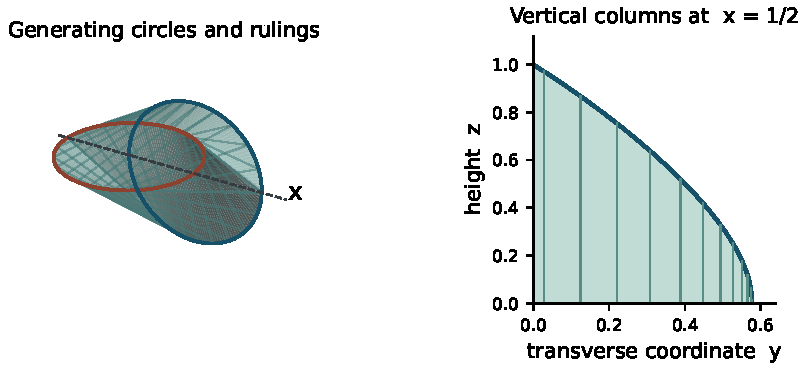
\includegraphics[width=.93\linewidth]{figures/geometry.pdf}
\end{center}
\noindent The area calculation goes back to Dirnböck and Stachel \cite{DS}; Huisman gives the elliptic forms of the volume and inertia \cite{Huisman}. Here a regular parametrization lets us compute the solid integrals by vertical columns. Three explicit exact differentials reduce them to \(K\) and \(E\). All limiting statements below have a reading as first-order inequalities on primitive recursive rational approximations. The accompanying Lean files and implementation plan distinguish the algebraic work from the remaining formal derivations.

\newpage
\sect{What the equalities mean in iPRA}\label{sec:ipra}
We use first-order intuitionistic logic, natural numbers, defining equations for primitive recursive (PR) functions, and quantifier-free induction. A rational is a sign, numerator, and positive denominator, encoded by natural numbers. Cross multiplication decides comparisons. Finite tuples, products, sums, and bounded searches are PR. A real constant in this paper is specified by a \emph{particular} PR approximation procedure with a proved modulus. There is no variable ranging over arbitrary functions or completed real sets.

Concretely, assign a rational center and an error radius at precision \(p\), with radius at most \(2^{-p}\), and prove that refinements give overlapping consistent enclosures (or that any two centers differ by at most the sum of the errors). An equality of two such descriptions means that their centers at precision \(p+2\) differ by at most \(2^{-p}\), for every \(p\). Substitution of a smaller mesh and interval rounding can always absorb fixed factors. The unit theorem uses only fixed procedures. For dyadic \(r,\rho>0\) scaling is uniform arithmetic. For specified real names for \(r,\rho\), the same assertion is a scheme with their moduli and rational upper bounds as inputs. A bound for dividing by \(V/r^3\) follows, for example, from \(K\ge\pi/2\) and \(E\ge\pi/4\).

\subt{A rational coordinate for angles.}
Use \(t\in[0,1]\) throughout. The following definitions give the entire analytic language needed in the geometric proof:
\[
 S=\frac{2t}{1+t^2},\qquad C=\frac{1-t^2}{1+t^2},\qquad
 \omega=\frac{2}{1+t^2},\qquad q=1-\tfrac34 S^2,\qquad w=\sqrt q .
\]
Write \(\dd\theta=\omega\,\dd t\), \(\Dth=\omega^{-1}\dd/\dd t\), and \(\int f\,\dd\theta=\int_0^1 f(t)\omega(t)\,\dd t\) when endpoints are suppressed. Then \(S^2+C^2=1\), \(\Dth S=C\), and \(\Dth C=-S\), by multiplication and differentiation of rationals. Define \(\arctan a=\int_0^a(1+u^2)^{-1}\dd u\) for \(0\le a\le1\) and \(\pi=4\arctan1\). Thus \(\theta=2\arctan t\) has length \(\pi/2\); \(S,C\) are its sine and cosine by the half-angle formulas. One may take the displayed rational formulas directly as the definitions in all the integrals, including \(K,E\). In particular \(1/4\le q\le1\).

\subt{Finite estimates behind the calculus.}
A nonnegative rational \(a\le B\) has a dyadic square-root enclosure from the greatest \(j\le 2^p(B+1)\) with \(j^2\le 2^{2p}a\) (round the bound upwards). The width is \(2^{-p}\). If an input also has uncertainty, evaluate the two endpoints; \(|\sqrt a-\sqrt b|\le\sqrt{|a-b|}\). For an \(L\)-Lipschitz function on an interval of length \(d\), every refined left sum differs from the coarse one by at most \(Ld^2/N\) on \(N\) equal cells. This follows by summing cell oscillations. Point evaluations of error \(\eta\) add at most \(d\eta\). Use common refinements for unequal grids. Iteration gives the rectangular version. All these inequalities are finite sums after denominators are cleared.

\newpage
\subt{Derivatives as finite remainders.}
In the calculations, \(f'\) means there is an effectively bounded remainder
\[
 |f(v)-f(u)-f'(u)(v-u)|\le H|v-u|^2 .
\]
For rational expressions and positive square roots this follows by expansion. If \(y=1/x\), the remainder after linearizing in \(\Delta x\) is \((\Delta x)^2/(x^2(x+\Delta x))\). If \(y=\sqrt x\), then
\(\Delta y-\Delta x/(2y)=-(\Delta y)^2/(2y)\). For products the additional remainder is the product of the increments. These identities also give the chain rule by substitution. For \(\arctan\), integrate the Lipschitz bound on \((1+u^2)^{-1}\) across one cell. Summing the remainder inequalities proves the fundamental theorem in the form
\[
 \left|\sum_i f'(u_i)\Delta u_i-f(b)+f(a)\right|
      \le H(b-a)\max_i\Delta u_i .
\]
Products give integration by parts by this same telescoping. For a monotone change \(y=g(t)\) with an \(L\)-Lipschitz integrand \(f\), the error of replacing each small integral by \(f(g_i)\Delta g_i\) is at most \(L\sum_i|\Delta g_i|^2\). More generally an oscillation bound on the composite along that cell suffices. This last form will apply at a vertical tangent.

Bounds can be computed from the formulas before sampling. For example, carry upper bounds for a function and its first two partial derivatives. Add componentwise, use the product rule twice for products, and use \(d^{-1}, B_1/d^2,2B_1^2/d^3+B_2/d^2\) for a reciprocal with lower bound \(d\) and derivative bounds \(B_1,B_2\). For a square root with root bounded below by \(e>0\), use \(B_1/(2e)\) and \(B_2/(2e)+B_1^2/(4e^3)\) for its derivative bounds. These bounds also cover mixed derivatives via the two product terms. The local remainder identities justify them without assuming a mean-value theorem for arbitrary functions. Use any rational upper bound for \(\sqrt B\), for instance \(1+B\). The chart uses only denominators bounded away from zero. Root evaluations at zero occur in describing the edges of a slice and use the square-root modulus above.

As a result, a requested precision determines a PR number of cells and precision for arithmetic evaluations. Specifically, for error budget \(\epsilon\) on a unit interval, \(N\ge 2(L+1)/\epsilon\) and evaluation radius at most \(\epsilon/2\) suffice. The same finite rules calculate a bound for each of the fixed larger rational expressions in the proof. Rational interval operations with lower denominator bounds or the displayed Lipschitz estimates assign working precision recursively to their inputs. Formally, induction in a finite sum is on partial integer sums and cross-multiplied bounds. A bounded family of hypotheses can be accumulated with a Boolean bounded conjunction. Universal precision and free object parameters are generalized \emph{after} the quantifier-free induction. This is the iPRA interpretation of the calculus notation used below.

\sect{A regular quarter of the surface}\label{sec:chart}
Take \(r=\rho=1\). The generating disks are centered at \((-1/2,0,0)\) in \(z=0\) and at \((1/2,0,0)\) in \(y=0\). Their convex hull agrees with that of the circles: a disk is filled by chords. One finite presentation of the hull takes all convex combinations of two disk points, then allows arbitrarily accurate approximation. Indeed, any finite rational convex combination groups its terms according to the disk; a zero group weight is decidable on finite data. Conversely convex combinations of disk points are approximated by combinations of circle points. Disk points have finite nets from the four reflected quarter-circle charts, a radial parameter in \([0,1]\), and their Lipschitz bounds. A radial disk segment lies between antipodal circle points.

\newpage
In the quadrant \(y,z\ge0\), set
\[
 a=\tfrac12-2q,\quad b=\frac{1-q}{2q},\quad
 Y=\sqrt3\,S w,\quad T=\sqrt3\,C,\quad Z=\frac{T}{2q},
 \qquad A=(a,Y,0),\quad B=(b,0,Z).
\]
With \(0\le s\le1\), write \(P(s,t)=(1-s)A+sB=(x,y,z)\). The factor \(D=b-a=2q+(2q)^{-1}-1\) satisfies
\[
 D-1=(2q-1)^2/(2q),\qquad \tfrac32-D=(1-q)(4q-1)/(2q).
\]
In particular \(1\le D\le 3/2\). Set \(c=2q-1\) and \(n=(-c,Y,T)\).
The relations \(c^2+Y^2=1,\ c^2+T^2=4q^2\) show that the two planar projections of \(n\) have lengths \(1,2q\). Each points along the radius of its disk at \(A,B\), respectively. Both supporting heights equal \(h=n\cdot A=n\cdot B=q+1/2\). Thus \(n\cdot U\le h\) throughout the hull. This proves that every ruling \(AB\) lies on its boundary.

To compute the area vector, let \(H=1+(2-3s)c=(1-s)(4q-1)+2s(1-q)\). Direct differentiation gives
\begin{equation}
 P_s\times\Dth P=\frac{H}{2qw}\,n,\qquad |n|=2w . \label{eq:cross}
\end{equation}
Here are algebraic steps to reproduce the computation. Put \(q'=-3SC/2\), \(w'=q'/(2w)\); then \(a'=-2q'\), \(b'=-q'/(2q^2)\), \(Y'=\sqrt3(Cw+Sw')\), \(Z'=-\sqrt3 S/(2q)-Tq'/(2q^2)\). The vectors to cross are \((D,-Y,Z)\) and \(((1-s)a'+sb',(1-s)Y',sZ')\). Substituting \(C^2=1-S^2\), \(w^2=1-3S^2/4\) in their three components gives \eqref{eq:cross}. The supplied symbolic check performs precisely these polynomial remainders. In particular \(H\ge0\) on the whole closed rectangle. Write \(J_z=TH/(2qw)\) for the \(z\)-component, the oriented Jacobian of the projection onto \(xy\) using \(s,\theta\).

\subt{Why the rulings cover the boundary.}
In the positive \(y\)-half of the \(xy\)-projection, the generating sets project to the first disk and a segment ending at \(x=3/2\); the other end of that segment is the disk center. The upper outline consists of the disk arc up to its tangent point \((0,\sqrt3/2)\), then the tangent segment to \((3/2,0)\). To verify this, the upper circular profile is concave (its hypograph on \(y\ge0\) is a half disk), and at \(x=0\) its slope is \(-1/\sqrt3\). Extending it by that tangent yields a concave majorant; every point on the extension is a convex combination of the two indicated endpoints. At any \(x\in[-3/2,3/2]\) the projected interval is therefore \(0\le y\le y_{\max}(x)\), where
\[
 y_{\max}(x)=
 \begin{cases}\sqrt{1-(x+1/2)^2},&x\le0,\\
 (3/2-x)/\sqrt3,&x\ge0.\end{cases}
\]
This pasted real function has the single expression
\(\sqrt{1-(\min(x,0)+1/2)^2}-\max(x,0)/\sqrt3\); the two-branch description requires no real comparison.

\newpage
\sect{The projected sweep, including the tangent seams}\label{sec:sweep}
For fixed \(x\), the admissible interval of \(t\) is given by \(a(t)\le x\le b(t)\), and the only possible weight is \(s_x(t)=(x-a)/D\). Both \(a,b\) increase with \(t\). Explicitly \(q_-\le q\le q_+\), where
\[
 q_-=\tfrac14-\tfrac12\min(x,0),\qquad
 q_+=\frac1{1+2\max(x,0)},\qquad
 t(q)=\frac{\sqrt{4(1-q)/3}}{1+\sqrt{(4q-1)/3}} .
\]
Thus the endpoints are \(\alpha=t(q_+)\) and \(\beta=t(q_-)\). Let \(Y_x(t)=(1-s_x(t))Y(t)\), \(Z_x(t)=s_x(t)Z(t)\). Substitution at the two endpoints gives \(Y_x(\alpha)=0,\ Y_x(\beta)=y_{\max}(x)\), and \(Z_x(\beta)=0\). For instance at the right edge of the projection with \(x\ge0\), \(q_-=1/4\) and \(s_x=2x/3\); with \(x\le0\), the upper endpoint is on the first circle with \(s_x=0\). These identities extend from rational \(x\) by the displayed moduli.

Holding \(x\) fixed in \(x=a+sD\) gives the crucial identity
\[
 \frac{\dd Y_x}{\dd t}=\frac{\omega J_z}{D}\ge0 .
\]
It follows by eliminating \(\dd s/\dd t\) from the two coordinate differentials. There is a quantitative inverse even where \(J_z\) vanishes. In the middle half of any admissible subinterval of length \(l\), \(S\ge t\ge l/4,\ C\ge1-t\ge l/4\). Since \(4q-1=3C^2\), \(2(1-q)=3S^2/2\), we have \(H\ge(3/2)(l/4)^2\). Also \(2qwD\le3,\ T\ge C,\ \omega\ge1\). Integrating on that middle half proves
\begin{equation}
 Y_x(t+l)-Y_x(t)\ \ge\ l^4/256 . \label{eq:inverse}
\end{equation}
For any required tolerance, sample the interval \([\alpha,\beta]\) at equally spaced parameters, evaluate \(Y_x\) with rational enclosures and take a sample of least approximate distance to the target \(y\). Monotonicity, both endpoint values, and the forward Lipschitz bound \(L\) imply a residual at most \(L/N+2\eta\) with sample error \(\eta\) (include the target error in \(\eta\)). This is a finite adjacent-cell argument on rational samples with interval slack. By \eqref{eq:inverse} any two candidates of residual \(\delta\) are within \((512\delta)^{1/4}\). This gives a PR name for the inverse, including a zero-length interval. In particular the height \(Z_x(t)\) is well defined on every projected column.

\subt{No extra height at a vertical tangent.}
Let \(U=(1-v)U_A+vU_B\) be a hull point, and compare it with a chart point \(P(s,t)\). A unit disk support in direction \(e\), \(|e|=1\), has deficit \(1-e\cdot d\ge |e-d|^2/2\) for every \(|d|\le1\). Applying this to the two disks, using \(2q\ge1/2\), gives
\[
 h-n\cdot U\ \ge\ \tfrac14\big((1-v)|U_A-A|^2+v|U_B-B|^2\big).
\]
If the planar projections are within \(\epsilon\) and \(U_z\ge P_z\), then \(h-n\cdot U\le\epsilon\), since \(|n_{xy}|=1,\ n_z\ge0\). The weighted square inequality shows that \(U\) is within \(2\sqrt\epsilon\) of \(P(v,t)\). Comparing \(x\) gives \(|v-s|\le\epsilon+2\sqrt\epsilon\), since \(D\ge1\). As \(Z\le1\), the excess height is at most \(\epsilon+4\sqrt\epsilon\). This inequality excludes every positive excess at equal projection, including limits of finite hull samples. Its derivation only needs the premise of a positive excess in an attempted violation. It works even when \(n_z=0\). Reflection in \(z=0\) and convexity fill the entire column between the two heights. Reflection in \(y=0\) completes the solid. The height is continuous jointly in \(x,y\). Indeed, for inputs within \(\delta\le1\), the endpoint formulas move by at most \(C_1\sqrt\delta\), using the root modulus. Clamp the old \(t\) to the new interval. The clamped value changes by at most \(C_1\sqrt\delta\), and its new \(Y_x\) misses the new target by at most \(C_2\sqrt\delta\), since \(Y_x\) has bounded partial derivatives in \(x,t\). By \eqref{eq:inverse} the new inverse parameter differs from the clamped one by at most \((256C_2\sqrt\delta)^{1/4}\). The same derivative bounds for \(Z_x\) give a PR height modulus of order \(\delta^{1/8}\). Thus a point strictly between the two graphs over the interior of the projection is interior to the solid. At the outside edge the two heights coincide. The boundary is exactly the four charts; their interiors are singly covered and their shared edges are curves.

\newpage
\sect{Finite geometric measurements}\label{sec:measure}
\subt{Area.}
Use the usual area of an injective smooth patch with piecewise smooth edges. Here it has a particularly direct arithmetic definition: divide the unit \((s,t)\)-square into \(N^2\) equal squares, split each along a diagonal, and sum the Euclidean triangle areas of the chart vertices. Take the sum for the four reflected patches. This definition also explains the area integral. At a vertex of a small square of side \(h_0\), the two triangle edge vectors are their first-order tangent displacements plus errors bounded by \(Ch_0^2\). The constant follows from the two-variable product and root rules of Section~\ref{sec:ipra}; a mixed term is bounded by varying one coordinate then the other. Taking a cross product introduces error at most \(C' h_0^3\) per triangle, since its tangent edges have length \(O(h_0)\). Taking a norm preserves this bound, even when the area vector is zero. Both triangles give half the parallelogram area to this accuracy. Summation gives \(O(1/N)\) with constants determined by the displayed chart. One may compute the vertices to error \(h_0^3\) with the same bound. Either choice of diagonal and further regular subdivisions give the same name. This is the elementary parametric definition of surface area on this finite atlas. On its interior the surface is singly covered and regular. Each edge curve is Lipschitz and its parameter strip has bounded area \(O(h_0)\), so the shared edges contribute zero.

By \eqref{eq:cross}, the answer on a unit oloid is
\[
 \mathcal A=4\int\!\int_0^1 H/q\,\dd s\,\dd\theta
       =4\int\left(1+\frac1{2q}\right)\dd\theta .
\]
For an explicit primitive of \(1/(2q)\), put \(U=C,\ W=S/2,\ w=\sqrt{U^2+W^2}\), and
\[
 F=2\arctan\!\left(\frac{W}{w+U}\right).
\]
The argument is in \([0,1]\), \(w+U\ge1/2\). Differentiating gives
\(\Dth F=(U\Dth W-W\Dth U)/w^2=1/(2q)\);
this follows by substituting \(\Dth w=(U\Dth U+W\Dth W)/w\) in the quotient rule. At \(t=0,1\) the values are \(0,\pi/2\). Hence \(\mathcal A=4(\pi/2+\pi/2)=4\pi\).

\subt{An independent solid-volume definition.}
For clarity, even the body whose moments we integrate has a rational inner and outer measurement. Let \(Q_0=[-1,1]^3\). Use dyadic mesh \(\eta\le1/16\) on the two planar disks and retain just the lattice points satisfying their rational disk inequalities. Let \(P_\eta\) be their rational convex hull. It contains \(\pm e_i/2\) for each coordinate unit vector and hence \(Q_0/8\). Shrink a disk radius vector by the factor \(1-3\eta\) and round both planar coordinates to the nearest grid point, keeping the other coordinate zero. The distance to the shrunken point is at most \(\sqrt2\,\eta\); the rounded point is in the disk and within \(5\eta\) of the original. Inclusions, with the outer distance in the maximum norm, follow by convexity:
\[
 P_\eta\ \subseteq\ \mathcal O\ \subseteq\
 P_\eta+\delta Q_0\ \subseteq\ (1+8\delta)P_\eta,\qquad \delta=5\eta .
\]
Both rational bounding polytopes refer to the same geometric oloid \(\mathcal O\) as the chart.

\newpage
For voxels of side \(h_0\le1/16\) in a fixed enclosing box, accept as inner a voxel with all vertices in \(P_\eta\); discard it as exterior if it misses \((1+8\delta)P_\eta\). Both predicates reduce to rational linear feasibility. Eliminate one unknown at a time by pairing each lower and upper bound, retaining constraints independent of that unknown; zero coefficients are decided rationally. Finite rational interval endpoints provide back-substitution witnesses. The variable count bounds the elimination loop, and each step at most squares the number of inequalities (up to an additive linear term), giving PR bounds on the finite procedure.

Every undecided voxel is in \((1+8\delta+8h_0)P_\eta\) and misses the interior of \((1-8h_0)P_\eta\). For the first assertion use the diameter \(h_0\) in the maximum norm. For the second, from a point in \((1-8h_0)P_\eta\) any voxel vertex lies in \((1-8h_0)P_\eta+h_0Q_0\subseteq P_\eta\). Thus their total volume is bounded by
\[
 \big[(1+8\delta+8h_0)^3-(1-8h_0)^3\big]\,64.
\]
Here \(64\) is the volume of the enclosing cube \([-2,2]^3\) for \(P_\eta\). This bound uses only finite rational polyhedral volume. For instance enumerate supporting facet planes through triples of vertices, triangulate each convex face in cyclic order, and cone to the origin (which is interior). Determinants give tetrahedral volumes; cutting these tetrahedra by rational planes gives finite additivity and the cubic scaling law. Intersections along polygonal boundaries have zero volume by the same subdivision or by slab bounds. Taking \(h_0=\eta=2^{-j}\) gives a PR modulus. For the polynomials \(1,y^2+z^2,x^2+z^2\), a fixed bound multiplies the undecided volume, and a Lipschitz bound times the voxel diameter controls interior sampling errors. This defines all three solid integrals independently of the surface formulas.

\subt{Integration by columns.}
Coordinate iteration agrees with the voxel definition: each inner or outer voxel indicator integrates to its volume by three one-dimensional sums; the product with the continuous weight is squeezed between its cell bounds. The preceding estimate makes the difference arbitrarily small. By Sections~\ref{sec:chart}--\ref{sec:sweep}, a column in \(y,z\ge0\) starts at zero and ends at the height \(z=P_z(s,t)\). Its integrated weights are respectively
\[
 z,\qquad z(y^2+z^2/3),\qquad z(x^2+z^2/3).
\]
On a fixed \(x\)-slice, partition \([\alpha,\beta]\). The increasing \(Y_x\) partitions the entire \(y\)-interval. The three top-column expressions along \(t\) are Lipschitz uniformly in \(x\), by \(D\ge1\) in \(s_x=(x-a)/D\). Over each induced \(y\)-cell their oscillation is at most \(L\Delta t\), by the inverse sweep. Multiplying by \(\Delta Y_x\) and summing bounds the total replacement error by \(Ly_{\max}\max\Delta t\). Replacing \(\Delta Y_x\) by \(Y'_x\Delta t\) costs \(O(\max\Delta t)\) by the finite remainder bound. In particular no reciprocal of \(J_z\) enters this substitution.

It remains to interchange \(x,t\) on \(a(t)\le x\le b(t)\). In a \(t\)-strip of width \(h_0\), the \(x\)-cells of width \(h_0\) which may cross either bounding graph have total length at most \(2(L_0+4)h_0\), where \(L_0\) bounds the two endpoint derivatives. This allows endpoint evaluations to error \(h_0/2\). Multiplication by the strip width and summation give lost area \(O(h_0)\). On the remaining rectangles one reorders finite sums. The integrand extends by the same rational formula for \(s_x\) to the enclosing rectangle with bounded derivatives. Finally substituting \(x=a+sD\) cancels \(D\) in \(Y'_x=\omega J_z/D\). We obtain, for any of the three displayed column weights \(G\),
\begin{equation}
 4\int\!\int_0^1 G(P(s,t))\,J_z\,\dd s\,\dd\theta . \label{eq:columns}
\end{equation}
The factor four comes from the two independent sign reflections.

\newpage
\sect{Reduction of the three solid integrals}\label{sec:reduce}
Define \(F_0=1,\ F_1=y^2+z^2/3,\ F_2=x^2+z^2/3\), enumerating the three column weights after the factor \(z\) is removed. The identities \(T^2=4q-1,\ z=sT/(2q)\) give
\[
 zJ_z=\frac{W_0}{w},\quad W_0=\frac{s(4q-1)H}{4q^2},\quad
 y^2=(1-s)^2\,4q(1-q),\quad z^2=\frac{s^2(4q-1)}{4q^2}.
\]
Set \(R_i(q)=4\int_0^1 W_0 F_i\,\dd s\); then the three answers in \eqref{eq:columns} are \(\int R_i(q)\,\dd\theta/w\). The \(s\)-integral is polynomial, with \(x=(1-s)(1/2-2q)+s(1-q)/(2q)\). Using \(\int_0^1s^j\,\dd s=1/(j+1)\) gives
\begin{align*}
 R_0={}& 2/q-1/(2q^2),\\
 R_1={}&-32q^2/15+12q/5-1/5-1/(3q)+3/(5q^2)-1/(4q^3)+7/(240q^4),\\
 R_2={}& 32q^2/15-16q/15+2/15-1/(10q)-5/(24q^2)+7/(24q^3)-7/(120q^4).
\end{align*}
For example \(4\int W_0\dd s=(4q-1)q^{-2}\int_0^1 s[1+(2-3s)c]\dd s=(4q-1)/(2q^2)\). The same three-line polynomial algorithm in \texttt{check\_identities.py} obtains the other rows from the coordinates.

\subt{Exact differentials.}
Put \(u=S^2=4(1-q)/3\). For a rational function \(g(q)\) define
\[
 \mathcal Lg=\left((1-2u)q-\tfrac34u(1-u)\right)g
              -\tfrac32u(1-u)q\,g'(q).
\]
The product rule, \(\Dth(SC)=1-2u\), and \(\Dth q=-3SC/2\) give
\[
 \Dth(SCw\,g(q))=\mathcal Lg/w.
\]
The factor \(SC\) vanishes at both ends; \(q\ge1/4\) bounds all denominators. To prove the desired values it suffices to check \(R_i=k_i+e_iq+\mathcal Lg_i\). The following polynomials specify all three witnesses.
\begin{center}
\renewcommand{\arraystretch}{1.24}
\begin{tabular}{@{}cccl@{}}\toprule
\(i\)&\(k_i\)&\(e_i\)&\(g_i(q)\)\\ \midrule
0 & \(2/3\)&\(4/3\)&\(-(2q-1)/(2q^2)\)\\
1 & \(-2/45\)&\(32/45\)&\(-(128q^4+16q^3+4q^2-18q+3)/(240q^4)\)\\
2 & \(-19/90\)&\(71/45\)&\((64q^4-78q^3-15q^2-3q+3)/(120q^4)\)\\ \bottomrule
\end{tabular}
\end{center}
These are identities of rational polynomials after clearing powers of \(q\). For example \(g_0=-q^{-1}+\tfrac12q^{-2}\) and
\(\mathcal Lg_0=2/q-1/(2q^2)-2/3-4q/3\).
For the last two rows the supplied checker expands the displayed expressions and returns zero for the numerator of each difference. Thus each is a finite equality of integer coefficients and a proof by ring arithmetic. The telescoping lemma from Section~\ref{sec:ipra} integrates the derivative to zero and yields exactly \(k_iK+e_iE\). This proves the three elliptic evaluations.

\newpage
\sect{Symmetry, scaling, and certified decimals}
For unit density the tensor at the origin has integrand \(|p|^2\delta_{ij}-p_i p_j\). Reflection of either \(y\) or \(z\) reverses the sign of a corresponding first moment and every mixed moment containing that variable to odd degree. The map \((x,y,z)\mapsto(-x,z,y)\) interchanges the disks, so the first \(x\)-moment also vanishes and \(\int y^2=\int z^2\). These symmetries may be applied to symmetric voxel sums directly. The origin is the center of mass since volume is positive. This proves diagonality and the equality of both transverse moments. Every transverse axis through the centroid consequently has the same moment. Scaling each coordinate by \(r\) multiplies triangle areas by \(r^2\), voxel volumes by \(r^3\) and their quadratic weights by \(r^2\). Uniform density supplies the additional factor \(\rho\), proving the full theorem.

\subt{Independent enclosures of the constants.}
Let \(a_0=1,\ a_j=a_{j-1}(2j-1)/(2j)=4^{-j}\binom{2j}{j}\). These are rationals in \([0,1]\). Integration by parts of \(S^{2j-1}C\), whose endpoint values vanish for \(j\ge1\), gives
\(\int S^{2j}\dd\theta=(\pi/2)a_j\). To justify the binomial expansions uniformly, put \(f(v)=\sum_{j\ge0}a_jv^j\) for \(0\le v\le3/4\). Its tail beyond \(N\) is at most \(4(3/4)^{N+1}\). The derivative tail is bounded by \(\sum_{j>N}j(3/4)^{j-1}=4(N+1)(3/4)^N+12(3/4)^N\). Hence termwise differentiation is justified by finite telescoping and these moduli. The coefficient recurrence gives \(2(1-v)f'=f\), so \(((1-v)f^2)'=0\). As \(f(0)=1,\ f\ge1\), we have \(f(v)=(1-v)^{-1/2}\). Multiplication by \(1-v\) gives \((1-v)^{1/2}\) with coefficient \(-a_j/(2j-1)\) for \(j\ge1\). Integrating the truncated polynomials at \(v=3S^2/4\) proves
\[
 \frac{2K}{\pi}=\sum_{j\ge0}a_j^2(3/4)^j,\qquad
 \frac{2E}{\pi}=1-\sum_{j\ge1}\frac{a_j^2(3/4)^j}{2j-1}.
\]
Both normalized errors after \(N\) are at most \(4(3/4)^{N+1}\). For the numerical implementation, \(\pi/2=8\arctan(1/5)-2\arctan(1/239)\). Indeed the slopes after doubling the angle of slope \(1/5\) twice are \(5/12,120/119\); subtracting the angle of slope \(1/239\) gives slope one in the first quadrant. The arctangent addition rule follows by differentiating the rational addition formula and evaluating at zero. Integrating the finite geometric expansion of \(1/(1+u^2)\) gives consecutive alternating bounds for each arctangent. The script uses only rational endpoints, with outward rounding for display. It proves the following enclosures:
\begin{center}
\begin{tabular}{@{}lll@{}}\toprule
Quantity for \(r=\rho=1\)& Lower bound & Upper bound\\ \midrule
\(\mathcal A\) & 12.5663706143591729 & 12.5663706143591730\\
\(V\) & 3.0524184684243748 & 3.0524184684243749\\
\(J_\ax\) & 0.7653502574931426 & 0.7653502574931427\\
\(J_\tr\) & 1.4555128734692003 & 1.4555128734692004\\ \bottomrule
\end{tabular}
\end{center}
The symbolic identities establish the equalities for every precision; the decimal calculation provides finite, separately reproducible bounds.

\newpage
\sect{A path to a kernel-checked iPRA derivation}\label{sec:lean}
The target in ProveIt \cite{ProveIt} is a closed sequent
\(\texttt{[]}\vdash_{\texttt{PRAAx}}\varphi\) for a concrete first-order sentence \(\varphi\).
Lean acts as the metatheory. A proof about a mathlib integral over real numbers would not by itself produce that sequent. The accompanying source separates three tasks.

\begin{enumerate}[leftmargin=1.5em,itemsep=5pt]
\item \textbf{Geometric algebra.} \texttt{ChartAlgebra.lean} uses ProveIt's \texttt{ZExp} language of integer polynomials and \texttt{derive\_imp}. Its variables \(d,c_0,a_0,b_0,s_0\) are scaled integers: \(c_0/d=c,\ a_0/d=Y,\ b_0/d=T,\ s_0/d=s\). The two circle identities become \(c_0^2+a_0^2=d^2,\ c_0^2+b_0^2=(d+c_0)^2\). The proposed sequents give the supporting heights, orthogonality, lengths and components of the cleared area vector. Each proof supplies a polynomial linear combination of the hypotheses. At rational mesh roots the circle residuals can be small but nonzero. Retain the displayed linear combinations, bound each multiplier on the chart, and carry the residual bounds when applying the exact identity to those samples.
\item \textbf{Elliptic reductions.} \texttt{EllipticReduction.lean} encodes the three unconditional polynomial identities of Section~\ref{sec:reduce}, homogenized at \(q=x/d\). The common denominator is positive on the chart. Recover rational identities by cross multiplication, then apply the finite telescoping inequality to the explicit function \(SCw g_i\). Its endpoint values are zero, so the quadrature defect is bounded by a constant divided by the mesh size.
\item \textbf{Numerical observations.} \texttt{Observations.lean} specifies mesh evaluations over \(\Q\) of the reduced geometry, the two elliptic integrals, and \(\pi\). At \(t=i/2^j\), compute \(q\) exactly and replace \(w\) by \(2^{-k}\lfloor\sqrt{\lfloor 2^{2k}q\rfloor}\rfloor\). The \(w\)-samples have lower bound \(1/2\) for \(k\ge1\). Form the weighted left sum with \(\omega\) and divide by \(2^j\). This gives a finite specification for each tag, independent of the elliptic series in the numerical checker.
\end{enumerate}

\subt{Object-language milestones.}
Encode a rational by integer difference and positive denominator, or by a PR tuple of naturals. Use fixed terms for \(+\), multiplication, cross-multiplied order, division by a positive rational, dyadic powers, bounded sums, and mesh roots. All program inputs to an induction are numbers or fixed terms. In particular the sum evaluator takes one of seven finite tags; no universal evaluator of PR programs is required. The following are concrete goals for completing the formalization.

\begin{enumerate}[leftmargin=1.5em,itemsep=4pt]
\item Derive the term-level root bracket from \texttt{Geometry.MeshBracket}. Lift the interval and remainder rules in Section~\ref{sec:ipra} along the finitely many expression trees. The reusable \texttt{Analysis.RiemannRefinement}, \texttt{Analysis.RiemannSumRules} and \texttt{Analysis.FiniteFTC} modules supply finite-sum inequalities and telescoping. Derive mixed parameter bounds via two successive one-variable estimates.
\item Define geometric observations from triangulated patches for area and rational inner/outer voxel sums for volume and moments, using Section~\ref{sec:measure}. Prove the support-gap and monotone-sweep inequalities by clearing the known positive denominators. For the inverse, let the search return the least index attaining the minimum rational residual; \eqref{eq:inverse} converts this residual into parameter precision. Compile the strip count, finite Fubini permutation, and the substitution estimates into a bound between geometric observations and their reduced grids. This is the geometric part of the unfinished formalization.
\item On the same grids prove the primitive identity for area and the three exact-differential identities. At common observation precision \(p+12\), state the four integer-linear defects
\[
 A-4\pi,\quad 3V-2K-4E,\quad 45J_\ax+2K-32E,\quad
 90J_\tr+19K-142E
\]
as signed rational intervals inside \([-2^{-p},2^{-p}]\). Here \(A,V,J_\ax,J_\tr\) are geometric observers evaluated to that precision, and \(K,E,\pi\) use separate reduced observers. Guard bits cover the sums of the absolute coefficients. Clear all positive denominators to get quantifier-free inequalities; take their conjunction and universally quantify \(p\). The paper's refinement estimates give the sizes of the intermediate grids as PR functions of \(p\), so the proof can specialize all witnesses before generalization.
\end{enumerate}

\subt{Checks and implementation status.}
The exact-arithmetic scripts test the chart identities, the three elliptic reductions, and the twelve integer-polynomial certificates transcribed from the Lean files. Another check starts with only the two generating circles: it approximates their convex hull by a polytope and partitions it into tetrahedra by joining each facet to the origin. For vertices \(0,v_1,v_2,v_3\), tetrahedral volume \(U\), and \(v=v_1+v_2+v_3\), its raw second-moment matrix is
\[
 \int pp^{\mathsf T}\,\dd V=\frac{U}{20}
 \left(vv^{\mathsf T}+\sum_{i=1}^3 v_i v_i^{\mathsf T}\right).
\]
This follows by integrating barycentric monomials on the unit simplex. At 768 equally spaced samples per circle the absolute discrepancies in area, volume, axial inertia, and transverse inertia were respectively \(9.58\,10^{-5},3.81\,10^{-5},1.69\,10^{-5},2.93\,10^{-5}\) or smaller. This floating-point calculation checks the choice of axes and the interpretation of the solid independently of the chart.

The area and moment equalities here are human proofs with explicit arithmetic interpretations. The provided Lean sources are a formalization scaffold. The new files have not been compiled in the preparation environment, and an end-to-end object-theory derivation of the geometry and analysis remains to be written. The companion roadmap identifies the pinned ProveIt modules and the bounds needed at each interface.

\begin{thebibliography}{9}\small\raggedright
\bibitem{DS} H. Dirnböck and H. Stachel, \emph{The development of the oloid}, Journal for Geometry and Graphics \textbf{1} (1997), 105--118. See the generator formulas (2), (4), and the area and volume calculations (31), (32).
\url{https://www.heldermann-verlag.de/jgg/jgg01_05/jgg0113.pdf}
\bibitem{Huisman} S. G. Huisman, \emph{The moment of inertia tensor of an oloid}, arXiv:2603.15145 (2026), in particular equations (2), (22), and (23).
\url{https://arxiv.org/abs/2603.15145}
\bibitem{ProveIt} V. Reshetnikov, \emph{ProveIt}, Logic/PrimitiveRecursiveArithmetic, including the \texttt{ConciseIPRA} and \texttt{IPRADerivations} Lean libraries. Pinned revision and module paths are provided in the archive's Lean roadmap.
\url{https://github.com/VladimirReshetnikov/ProveIt/tree/main/Logic/PrimitiveRecursiveArithmetic}
\end{thebibliography}
\end{document}
